\chapter{Exponential Functions}
\label{ch:expofunc}

\chapquote{The greatest shortcoming of the human race is our inability to understand the exponential function.}{Albert A. Bartlett\\American physicist}

%\begin{quote}
%The greatest shortcoming of the human race is our inability to understand the exponential function.
%\par\hfill -- Albert A. Bartlett, American physicist
%\end{quote}

Every chapter should have a lead paragraph -- even just a short one -- that appears before the first heading. This is a placeholder paragraph which will at some point be replaces by actual content.

%%% Good somewhere?
%\begin{boxedexplore}[Startup Exploration: The Water Lily]
%On Fran\c{c}ois's farm, there is a pond with awater lily leaves floating on its surface. If the lily is allowed to grow without interference, it will eventually cover the surface of the pond, blocking the light and starving the other plants that live in the water.
%
%Over the years Fran\c{c}ois has learned that the lily population doubles in size every day, and that it takes 30 days to cover the surface of the pond. At the start of a new growing cycle, Fran\c{c}ois tells Ivan to monitor the situation and to cut the lily back when it covers half of the pond. On what day should Ivan do this?
%\end{boxedexplore}

%% % % % % % % % % % % % % % % % % % % % % % % % % % % % % % % % % % % % % % % % 
\section{Exponential Relationships}
\label{sec:exporelationships}

\begin{boxedexplore}
YeardleighCorp genetic engineers have developed a new kind of fast-growing, nutrient-rich seaweed for the turtle pens. The length of a strand of this seaweed doubles every day.

Scientists measure a particular strand of seaweed to be 15 centimeters long. How long will this strand be in 1 day? 2 days? 3 days? How long was this strand 1 day ago? 2 days ago? 3 days ago?
\end{boxedexplore}

We are told that the seaweed doubles in length each day, so after one day the strand will be 30 cm long. Continuing the doubling pattern, the strand will be 60 cm after two days, and then 120 cm after three days.

We can analyze this doubling pattern using the skills we learned in \cref{ch:sequences}. The recursive rule rule for the length of the strand is: ``start with 15 centimeters, and multiply the previous value by 2''. If we think of the starting length as the ``stage 0'' length, then we can write a rule for the pattern:
\[L(t) = 15 \cdot 2^t,\]
where $L(t)$ represents the length of the seaweed strand in centimeters after $t$ days.

To make this doubling pattern go ``backwards in time'', we must divide by 2. One day ago the strand must have been 7.5 cm long, since doubling this value get us to the original measurement of 15 cm. Going further, the strand was 3.75 cm long two days ago, and 1.875 cm long three days ago.

We can organize our data in a table, and make a scatter plot. Note that we use negative numbers to represent days in the past (days before day 0, on which we took the starting measurement).

\begin{minipage}[c]{0.5\textwidth }
	\centering
	\begin{tabular}{|C{2cm}|C{2cm}|}
	\hline
	\text{\footnotesize Time (days)} & \text{\footnotesize Length (cm)}\\
	t & L(t)\\\hline
	-3 & 1.875\\
	-2 & 3.75\\
	-1 & 7.5\\
	0 & 15\\
	1 & 30\\
	2 & 60\\
	3 & 120\\\hline
	\end{tabular}
\end{minipage}%
%
\begin{minipage}[c]{0.5\textwidth }
	\centering
%	\resizeplot{-4}{0}{4}{120}
	\begin{tikzpicture}[scale=1.2]
	\begin{axis}[
			clip=false,
			width=0.625\linewidth,
			height=0.625\linewidth,
			axis lines = middle,
			axis line style={thick, <->, shorten >=-10pt, shorten <=-10pt},
			xlabel={$t$},
			ylabel={$L(t)$},
			grid=both,
			%xlabel near ticks,
			minor xtick={-4,...,4},
			%ylabel near ticks,
			minor ytick={0,10,...,120},
		]
%		\addplot[algcurve, ->, red, domain=0:50] (\x,4.5*x+270);
%		\addplot[algcurve, ->, green!50!black, domain=0:42] (\x,12*x);
		\addplot[algpoints, blue, mark size=2] coordinates
			{(-3,1.875)(-2,3.75)(-1,7.5)(0,15)(1,30)(2,60)(3,120)};
%		\draw[green!50!black] (axis cs:20,200,0)
%			node[rotate=50.2]{\large$y=12.00x$};
%		\draw[red] (axis cs:15,365,0)
%			node[rotate=24.2]{\large$y=4.50x+270$};
%		\draw (axis cs:36,432,0) node[below right]{\large$(36,432)$};
	\end{axis}
\end{tikzpicture}
\end{minipage}
\medskip

From these three representations, it is clear that we have an exponential relationship on our hands: The rule has the independent variable used as an exponent, the table shows repeated multiplication, the graph as that smooth J-like shape that we saw in \cref{ch:functions}.

A new wrinkle that comes up here, though, is the idea of using negative numbers as the exponent. If we're right about our rule, for example, then it must be that \[15 \cdot 2^{-2} = 3.75,\]
which is not an obvious statement! Let's look more closely at this idea.

% % % % % % % % % % % % % % % % % % % % % % % % % % % % % % % % % % % % % % % % 
\subsection{Negative Exponents}
\label{sec:exponegative}

Recall that when we talk about exponents and exponential expressions, we're talking about expressions of the form: $a^b$. This is read ``$a$ to the power of $b$'' or ``$a$ to the $b^{\text{th}}$ power''. In such an expression, $a$ is called the \textit{base} and $b$ is called the \textit{exponent}. Since $a$ is the base, we call the whole thing a \textit{power of $a$}.

One interpretation of this expression, as we have seen, is as repeated multiplication:
\[a^b = \underbrace{a \cdot a \cdot a \cdot \dotsm \cdot a}_{\text{$b$ times}}\]
This representation is a bit limited --- it really only works when the exponent $b$ is a positive integer --- but it is still helpful for gaining some intuition about how exponents work.

For clarity, we will name the different forms of the exponential expression. We will use the term ``exponent form'' to describe $a^b$, and  ``expanded form'' to describe the form where the multiplication is written out. So, for example, $12^4$ is in exponent form, and \[12\cdot12\cdot12\cdot12\] is the same number written in expanded form. Of course, if the base is a number, we can compute this value: \[12^4 = 12\cdot12\cdot12\cdot12 = 20\,736.\] This last value (the number) is in ``standard form'' or ``decimal form''. Expressions like $a^b$ have no decimal form until we know what numbers $a$ and $b$ represent.

\subsection{Extending Repeated Multiplication}

Recall that in \cref{sec:orderofops} we mentioned a rule for using zero as an exponent:

\begin{boxeddef}[Zero Exponent]
For any nonzero real number $a$, \[a^0 = 1.\]
\end{boxeddef}

Our goal now is to extend this idea to include exponents that are negative integers. We'll do this informally by looking at exponential patterns. We'll start with a table that just shows the non-negative integral powers of 5:

\begin{center}
\begin{tabular}{C{1.5cm}L{2.75cm}L{1.5cm}}
5^5		 &  =~ 1\cdot5\cdot5\cdot5\cdot5\cdot5	& =~ 3125\\
5^4		 &  =~ 1\cdot5\cdot5\cdot5\cdot5			& =~ 625\\
5^3		 &  =~ 1\cdot5\cdot5\cdot5					& =~ 125\\
5^2		 &  =~ 1\cdot5\cdot5						& =~ 25\\
5^1		 &  =~ 1\cdot5								& =~ 5\\
5^0		 &  =~ 1									& =~ 1\\
\end{tabular}
\end{center}

Moving ``upwards'' in this table involves multiplication by 5. Each new row that we pile on top of the table would add 1 to the exponent and put a new factor of 5 in the middle column. If moving upwards in the table means multiplication by 5, then moving ``downwards'' in the table must mean division by 5, or in other words, multiplication by $\frac{1}{5}$ (the reciprocal of 5).

So, we can extend the table downwards, as shown below. We take away 1 from the exponent in each step, and introduce repeated multiplication by $\frac{1}{5}$.

\begin{center}
\begin{tabular}{C{1.5cm}L{2.75cm}L{1.5cm}}
5^5		& =~ 1\cdot5\cdot5\cdot5\cdot5\cdot5		& =~ 3125\\
5^4		& =~ 1\cdot5\cdot5\cdot5\cdot5			& =~ 625\\
5^3		& =~ 1\cdot5\cdot5\cdot5					& =~ 125\\
5^2		& =~ 1\cdot5\cdot5							& =~ 25\\
5^1		& =~ 1\cdot5								& =~ 5\\
5^0		& =~ 1										& =~ 1\\
5^{-1}	& =~ 1\cdot\frac{1}{5}						& =~ \frac{1}{5}\\
5^{-2}	& =~ 1\cdot\frac{1}{5}\cdot\frac{1}{5}		& =~ \frac{1}{25}\\
5^{-3}	& =~ 1\cdot\frac{1}{5}\cdot\frac{1}{5}\cdot\frac{1}{5}
& =~ \frac{1}{125}\\
5^{-4}	& =~ 1\cdot\frac{1}{5}\cdot\frac{1}{5}\cdot\frac{1}{5}\cdot\frac{1}{5}
& =~ \frac{1}{625}\\
5^{-5}	& =~ 1\cdot\frac{1}{5}\cdot\frac{1}{5}\cdot\frac{1}{5}\cdot\frac{1}{5}\cdot\frac{1}{5}
& =~ \frac{1}{3125}\\
\end{tabular}
\end{center}

There are a number of important patterns to see in this table. For example, the pattern ``divide by 5 as we move downwards in the table'' helps us to explain why $5^0 = 1$. Also note which numbers in the table are reciprocals of one another. This suggests a general rule for working with negative exponents.

\begin{boxeddef}[Negative Exponents]
For any nonzero real number $a$, and any positive integer $n$, \[a^{-n}=\frac{1}{a^n}.\]
In other words, $a^{-n}$ is the reciprocal of $a^n$ (the base raised to the opposite power).
\end{boxeddef}

One aspect of negative exponents that can be confusing is that the negative exponent does not change the sign of the evaluated expression. For example, all of the numbers in the table above are positive numbers, even though they have a negative number in the exponent!

Also note that this rule explicitly states that $a$ must be a \textit{nonzero} real number. Can you explain why is this important? Why can't we raise 0 to a negative exponent?

\begin{boxedex}
Write each of the following in standard form (as a fraction in lowest terms).

\begin{center}
\begin{tabularx}{0.6\textwidth}{XXX}
(a)~ $36^{-1}$
&
(b)~ $2^{-6}$
&
(c)~ $\left(\dfrac{3}{4}\right)^{-2}$
\end{tabularx}
\end{center}

\exsoln\ In each case, we can take the reciprocal of the number and raise it to the positive version of the power, so \[36^{-1} = \left(\frac{1}{36}\right)^1 = \frac{1}{36}\]
The next two require a bit more computation, but the idea is the same. Problem (b) becomes:
\[2^{-6} = \left(\frac{1}{2}\right)^6 = \left(\frac{1}{2}\right)\left(\frac{1}{2}\right)\left(\frac{1}{2}\right)\left(\frac{1}{2}\right)\left(\frac{1}{2}\right)\left(\frac{1}{2}\right) = \frac{1}{64}\]
And problem (c) becomes:
\[\left(\frac{3}{4}\right)^{-2} = \left(\frac{4}{3}\right)^2 = \left(\frac{4}{3}\right)\left(\frac{4}{3}\right) = \frac{16}{9}\]
\end{boxedex}

It pays to take time when working on problems like this. Consider the next examples carefully!

\begin{boxedex}
Rewrite each of the following expressions in an equivalent form that uses only positive exponents.
\begin{center}
\begin{tabularx}{0.4\textwidth}{XX}
(a)~ $7m^{-2}$
&
(b)~ $\dfrac{3^{-1}}{~4~}$
\end{tabularx}
\end{center}

\exsoln\ We might make a mistake if we rush into these expressions too quickly. Recall that we have to be clear about exactly what an exponent is attached to. In the first expression, the exponent applies only to the $m$, not the whole expression (there are really two operations here --- what are they?). And so,
\[7m^{-2} = 7\left(\frac{1}{m}\right)^2 = \left(\frac{7}{1}\right)\left(\frac{1}{m}\right)\left(\frac{1}{m}\right) = \frac{7}{m^2}\]
In the second expression, the exponent applies only to the 3 in the numerator, and not the whole fraction (there's a subtle grouping symbol here --- what is it?). This expression becomes:
\[\dfrac{3^{-1}}{~4~} = \dfrac{\tfrac{1}{3}}{~4~} = \frac{1}{3}\div{4} = \left(\frac{1}{3}\right)\left(\frac{1}{4}\right) = \frac{1}{12}\]
\end{boxedex}

The second expression went through a rather ugly, fraction-in-a-fraction phase, but don't worry: we'll soon learns some simplification rules that will help us make quick work of expressions like these.

\subsection{Smaller and Smaller}

An interesting consequence of this negative exponent business is that we get a progression of numbers that get smaller and smaller, but never disappear. For example, in the sequence of powers of 5 above, as $n$ gets larger, the number $5^n$ grows huge! By the time $n=10$, the number $5^{10}$ is nearly 10 million.

This means that $5^{-10}$ is 1-over-something-close-to-10-million. That number is incredibly small. But note that it is still a positive number. As $n$ gets larger and larger $5^{-n}$ gets closer and closer to zero, but never actually reaches zero. There is always a tiny fraction which makes the number $5^{-n}$ a wee bit greater than zero.

If we look at the graph of $y=5^x$, we see that the curve flattens out as we look to the left, along the negative $x$-axis. The line approaches 0 but never reaches it. To capture this idea, we say the graph as a \textit{horizontal asymptote} at $x=0$.\footnote{We'll learn more about asymptotes, and other unusual graph behavior, at the very end of this course and in algebra 2.}

%\resizeplot{-3}{-8}{7}{1}
\begin{center}
\begin{tikzpicture}
	\begin{axis}[
			clip=false,
			width=0.625\linewidth,
			height=0.625\linewidth,
			axis lines = middle,
			axis line style={thick, <->, shorten >=-10pt, shorten <=-10pt},
			xlabel={$x$},
			ylabel={$y$},
			grid=both,
			%xlabel near ticks,
%			minor xtick={-4,...,4},
			%ylabel near ticks,
%			minor ytick={0,10,...,120},
		]
		\addplot[algcurve, blue, domain=-5:5] (\x,5^\x) node[right]{$y=5^x$};
	\end{axis}
\end{tikzpicture}
\end{center}

We can also see how steep the curve gets as we go along the positive $x$-axis. An important aspect of understanding exponential relationships is understanding this dual nature: incredibly steep on one end, incredibly flat on the other.

\addtodoitem{Idea: include Zeno's paradox here? Or as a journal prompt or activity of some kind?}

\begin{boxedexplore}[Startup Exploration: Zeno's Paradox]
A paradox is a statement from which we can follow a logical path of reasoning to an impossible of self-contradictory end.

The ancient Greek philosopher Zeno proposed a set of paradoxes about motion. One of these says:

{\centering A moving object must arrive at the half-way point on its path before it reaches its goal.}

This seems like an obvious statement, right? If you shoot an arrow at a target, the arrow must go half of the distance between you and the target before is goes the whole way to the target!

Let's call the half-way point ``point A'' and suppose the arrow is there. Now consider this: before the arrow can fly to the target from point A, it has to go half of the remaining distance. So, the arrow arrives at a point three-fourths of the way along the path. Let's call this point B.

Now, before the arrow can go from point B to the target, it has to go half-way to the target. Now it's seven-eighths of the way there.

Before it can cover the remaining distance it has to cover half of the remaining distance\ldots\ and this is always true. So, Zeno says, the result is that the arrow never actually reaches the target: there's always a little but more to go!

In fact, it's even worse! Before the arrow can go halfway to the target, the arrow has to go one-fourth of the way. But before it can do that, it has to go one-eighth of the way. In fact, before the arrow can cover any distance, it has to cover half of that distance\ldots\ and so the arrow never moves in the first place!

Zeno says that movement is impossible, since the above statement about ``going half-way'' is true. Of course, we know that movement is possible! We do it all the time! This contradiction is what makes the paradox.

Many resolutions to the paradox have been proposed over the year, but it wasn't until the 19th century --- around 2000 years after Zeno lived --- that mathematics had a clear and rigorous solution to the paradox.

What do you think about these ideas? 
\end{boxedexplore}

% % % % % % % % % % % % % % % % % % % % % % % % % % % % % % % % % % % % % % % % 
\section{Exponential Growth}
\label{sec:expogrowth}

\begin{boxedexplore}[Extended Exploration: A Problem With Turtles]
\addtodoitem{LINK.}
\end{boxedexplore}

\begin{boxedexplore}[Startup Exploration: Cantor Set]
German mathematician Georg Cantor suggested a way to construct a very interesting set of numbers. We start in Stage 0 with a line segment covering the interval from 0 to 1 on the number line. The recursive procedure is to remove the middle third from each of the line segments in the previous step. The first few iterations are shown.

\newlength{\cantorht}
\setlength{\cantorht}{0.25cm}
\begin{center}
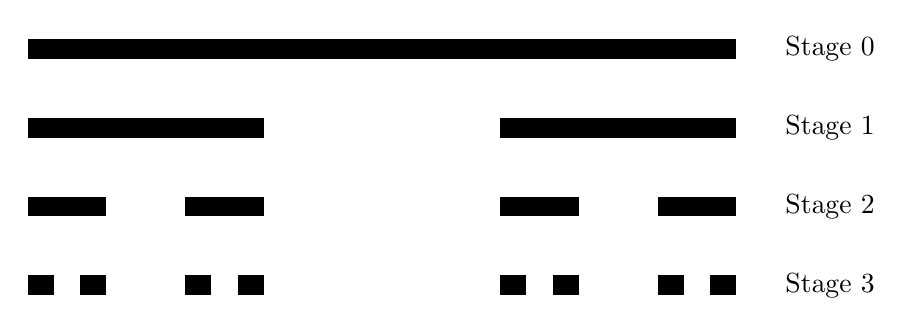
\begin{tikzpicture}
	\draw (9.5, 0.5\cantorht) node[right]{Stage 0};
	\fill (0,0) rectangle (9, \cantorht);

	\begin{scope}[yshift=-1cm]
		\draw (9.5, 0.5\cantorht) node[right]{Stage 1};
		\foreach \x in {0,6}
			\fill (\x,0) rectangle (\x+3, \cantorht);
	\end{scope}

	\begin{scope}[yshift=-2cm]
		\draw (9.5, 0.5\cantorht) node[right]{Stage 2};
		\foreach \x in {0,2,6,8}
			\fill (\x,0) rectangle (\x+1, \cantorht);
	\end{scope}

	\begin{scope}[yshift=-3cm]
		\draw (9.5, 0.5\cantorht) node[right]{Stage 3};
		\foreach \x in {0,2, 6, 8} {
			\fill (\x,0) rectangle (\x+1/3, \cantorht);
			\fill (\x+2/3,0) rectangle (\x+1, \cantorht);
		}
	\end{scope}
\end{tikzpicture}
\end{center}

Let $f(x)$ represent the number of segments in stage $x$ of this construction. Write an equation for $f(x)$. How many segments are in stage 10 of the figure? What is the first stage to contain more than 100,000 segments?

\textit{Bonus puzzler.} The set of points from the original line segment that are not deleted at any step of the (infinite) process is called the \textit{Cantor ternary set}. Can you give an example of a point that is in this set? What can we say about the points that survive this process?
\end{boxedexplore}

\subsection{Modeling Exponential Growth}

The number of segments in the construction of the Cantor set doubles each time, so the pattern follows the rule ``start with 1, multiply the previous value by 2''. We can write out the repeated multiplication in expanded form, or use an exponent.

\begin{center}
\renewcommand{\arraystretch}{1.1}
\begin{tabular}{|C{1.75cm}|C{1.5cm}|L{2.5cm}|C{1.5cm}|}
\hline
\text{Stage No.} & \multicolumn{3}{c|}{No. of Segments}\\
\hline
0 & 1 & 1 & 1\cdot2^0\\
1 & 2 & 1\cdot2 & 1\cdot2^1\\
2 & 4 & 1\cdot2\cdot2 & 1\cdot2^2\\
3 & 8 & 1\cdot2\cdot2\cdot2 & 1\cdot2^3\\
4 & 16 & 1\cdot2\cdot2\cdot2\cdot2 & 1\cdot2^4\\
\hline
\end{tabular}
\renewcommand{\arraystretch}{1}
\end{center}

If we compare the first and last columns in the table, we can see that the explicit rule for the number of segments depends only on the stage number. We have the rule \[f(x)=1\cdot2^x.\]
Now that we have an equation, it's quite easy to find the number of segments in stage 10 of the figure: \[f(10) = 1\cdot2^{10} = 1024.\]

To determine the stage in which the figure first has more than 100,000 segments, we need to solve the following equation for $x$: \[100,000 = 2^x\] Hmm. This is a bit of a problem, since we don't have a POE that helps us to get $x$ out of the exponent.\footnote{We don't have such a POE \textit{yet}. There are POEs that will help us in situations like this, but they're going to have to wait until algebra 2, when we will learn about the concept of a \textit{logarithm}.} For now, we'll have to settle for doing a bit of detective work to find this value.

One approach is to use technology. With a graphing calculator or other tool that will display a table of values when given a rule, we can punch in the rule and search through the table for the first row in which the number of segments exceeds 100,000.

If we're working by hand (or working with a regular four-function calculator) we can extend our table manually, or adopt an educated guess-check-revise strategy. In this case, we work forward from $f(10)=1024$. We don't have to hunt for very long:
\[\begin{aligned}
f(11) &= 2048\\
f(12) &= 4096\\
f(13) &= 8192\\
f(14) &= 16\,384\\
f(15) &= 32\,768\\
f(16) &= 65\,536\\
f(17) &= 131\,072\\
\end{aligned}\]
So, stage 17 is the first stage to contain more than 100,000 segments. Are you surprised by this? The figure grows from around 1000 segments in stage 10 to more than 100 times that number of segments less than 10 stages later! Surprising results like this are part of what make exponential relationships so much different from linear relationships.

\subsection{Extending the Growth Model}
Suppose we build an equilateral triangle in which each side is a Cantor segment. Then we let $g(x)$ represent the number of segments in stage $x$ of this new figure. Let's try to answer the same questions as above: how many segments in stage 10, and in what stage will the number of segments first exceed 100,000?

\begin{center}
\begin{minipage}{0.32\textwidth}
	\centering
	Stage 0
	\par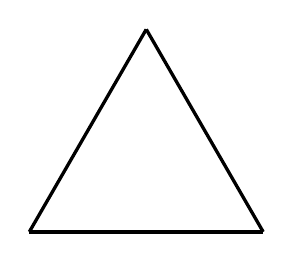
\begin{tikzpicture}[scale=0.33]
		\draw[very thick] (0,0) -- (9,0);
		\draw[very thick, rotate=60] (0,0) -- (9,0);
		\draw[very thick, xshift=9cm, rotate=120] (0,0) -- (9,0);
	\end{tikzpicture}
\end{minipage}
%
\begin{minipage}{0.32\textwidth}
	\centering
	Stage 1
	\par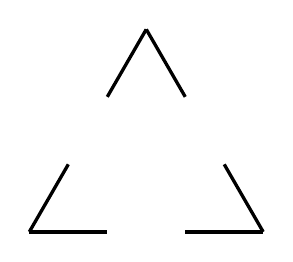
\begin{tikzpicture}[scale=0.33]
		\foreach \x in {0,6} {
			\draw[very thick] (\x,0) -- (\x+3,0);
			\draw[very thick, rotate=60] (\x,0) -- (\x+3,0);
			\draw[very thick, xshift=9cm, rotate=120] (\x,0) -- (\x+3,0);
		}
	\end{tikzpicture}
\end{minipage}
%
\begin{minipage}{0.32\textwidth}
	\centering
	Stage 2
	\par\begin{tikzpicture}[scale=0.33]
		\foreach \x in {0,2,6,8} {
			\draw[very thick] (\x,0) -- (\x+1,0);
			\draw[very thick, rotate=60] (\x,0) -- (\x+1,0);
			\draw[very thick, xshift=9cm, rotate=120] (\x,0) -- (\x+1,0);
		}
	\end{tikzpicture}
\end{minipage}
\end{center}

The only difference here is that we've changed the initial number of segments. Now, we have the rule ``start with 3, multiply the previous value by 2''. The updated table is shown below.

\begin{center}
\renewcommand{\arraystretch}{1.1}
\begin{tabular}{|C{1.75cm}|C{1.5cm}|L{2.5cm}|C{1.5cm}|}
\hline
\text{Stage No.} & \multicolumn{3}{c|}{No. of Segments}\\
\hline
0 & 3 & 3 & 3\cdot2^0\\
1 & 6 & 3\cdot2 & 3\cdot2^1\\
2 & 12 & 3\cdot2\cdot2 & 3\cdot2^2\\
3 & 24 & 3\cdot2\cdot2\cdot2 & 3\cdot2^3\\
4 & 48 & 3\cdot2\cdot2\cdot2\cdot2 & 3\cdot2^4\\
\hline
\end{tabular}
\renewcommand{\arraystretch}{1}
\end{center}

Notice how we only need to change one part of the first rule that we wrote: \[g(x)=3\cdot2^x\]
To find the number of segments in stage 10, we compute $g(10) = 3\cdot2^{10} = 3072$. Then, we do some detective work to find the stage number in which we first exceed 100,000 segments. Stage 15 is close with $g(15)=98\,304$, but it is stage 16 that first breaks the barrier: $g(16) = 196\,608$.

\subsection{Exponential Equations}

If we summarize our findings from the explorations above, we have the ``general form'' of an exponential function.

\begin{boxeddef}[General Form of the Exponential Function]
A equation of the form \[f(x)=a \cdot b^x\] is an exponential function if $a\neq0$, $b\neq1$, and $b>0$. The constant value $a$ is the \textit{initial value} of the function (when $x=0$). The constant value $b$ is called the \textit{constant multiplier}. 
\end{boxeddef}

Note that there are some constraints placed on the ``legal'' values of $a$ and $b$. Why do we need these restrictions?

Consider what happens when $a=0$. In this scanario, the function $f(x)=ab^x$ degenerates to $f(x)=0$. That isn't an exponential function, it's a horizontal line along the $x$-axis! Simiarly, if $b=1$, then $f(x)=ab^x$ degenerates into $f(x)=a$. That's a horizontal line through the point $(0,a)$!

What about the restriction $b>0$? Consider what happens when $b$ is negative, for example $f(x)=(-2)^x$. When $x$ is an even integer, $f(x)$ is positive. When $x$ is an odd integer, $f(x)$ is negative. This back-and-forth means that the graph doesn't have the same smooth curving shape that we associate with the exponential family. Plus, we haven't even talked about values of $x$ that are not integers! Those have all sorts of other problems!

When $b$ is greater than 1, we have a situation like the ones we have seen in this chapter, called \textit{exponential growth}. Note that $b$ could also be a positive fraction: numbers between 0 and 1 are allowed. In the case that $b$ is a fraction, the exponential behaves a bit differently. We'll study this situation, called \textit{exponential decay}, in \cref{sec:expodecay}.


% % % % % % % % % % % % % % % % % % % % % % % % % % % % % % % % % % % % % % % % 
\section{Percent Change}
\label{sec:expopercentchange}

Earlier explorations have involved an amount doubling as time went by. But what if we have a quantity that grows at a different rate? For example, the United Nations estimates that the population of the Earth will grow by approximately 0.77\% per year between now and 2050. How do our rules have to change to accomodate an arbitrary rate of growth?

\begin{boxedexplore}[Startup Exploration: Hermine's Choice]
Hermine is shopping for a mother's day gift. The vase she wants to buy is on sale for 25\% off. She also has a 10\% off coupon that can be applied to any item in the store. The store manager agrees that she can use both discounts, and gives her two options: \textit{Option 1}: Take 25\% off the full price of the vase, then apply the coupon to the discounted price. \textit{Option 2}: Apply the 10\% coupon to the full price of the vase, and then take 25\% off the discounted price.

Which option should Hermine choose? Why?

Later, Hermine told Bob this story. He said, ``Wow! 35\% off! You got a great deal!'' How would you respond to Bob?
\end{boxedexplore}

In \cref{ch:proportions}, we discussed the percent proportion:
\[\frac{\text{part}}{\text{whole}} = \frac{\text{percent}}{100}.\]
A key use of percents, as we saw, is to make clear and accurate mathematical comparisons. One comparison that is often illuminating is to compare a certain quantity with itself. If the quantity has increased or decreased over time, we may want to know \textit{by what percent} has it changed?

To calculate a percent change, we compare the amout that a quantity has changed to its starting value. In other words, 
\[\frac{\text{amount of change}}{\text{original amount}} = \frac{\text{percent change}}{100}.\]
If we wish to isolate percent change, we can multiply both sides by 100.

Of course, a value may grow larger or smaller, and so we must remember to be clear and describe the percent change as either a ``percent increase'' or ``percent decrease''.

\begin{boxedex}
Yeardleigh gives Hermine \$300 worth of YeardleighCorp stock as a birthday gift. After one month, the value of YeardleighCorp stock had increased by 15\%. How much were Hermine's shares worth at that point?

After two months, Hermine's shares are worth \$240. What is the percent change from her original \$300 gift? What is the percent change from the value of her shares after one month?

\exsoln\ To compute the value after one month, we find \%15 of the value: $300(0.15) = 45$, and then we add this on to find the new total value. So, after one month Hermine's shares are worth $300 + 45 = 345$ dollars.

Since the stock value goes down in the second month, we're looking for percent decrease. The drop from the original value is $300-240=60$ dollars. We compare this to the original price to find the percent change from that price: \[\frac{300}{60} = 0.2 = 20\%\]
We can make the same comparison with the price after one month. The amount of the change is $345-240=105$ dollars, so the percent change from that price is: \[\frac{105}{345} \approx 0.304 \approx 30\%\]
So Hermine's shares have undergone a 20\% decrease from their starting value, and a 30\% decrease from their price one month ago.
\end{boxedex}

Note that to calculate the percent increase we found 15\% of 300 and then added that on to the original 300. So the new amount is \[300 + 300(0.15).\] We can apply the distributive property to this and get \[300(1+0.15) = 300(1.15).\] If we interpret this as a percent question in its own right, we are saying that the new value is 115\% of the original value. This might seem like an unusual statement, but it makes sense: we have 100\% of the amount (all of what we started with) and then we add on an additional 15\%.

Now consider the case of a percent decrease, such as Hermine's discount coupon in the startup exploration. If Hermine wants to buy a vase that costs \$75 and has a 10\% off coupon, we can find 10\% of the value of the vase and subtract that from the original value: \[75 - 75(0.10)\] Applying the distributive property as we did above, we have: \[75 - 75(0.10) = 75(1-0.10) = 75(0.90)\] This makes sense, too: if Hermine gets 10\% off the price of the vase, then she is only paying 90\% of the original price. Armed with these ideas, we can determine which option Hermine should choose in the startup exploration.

\begin{boxedex}[Explaining the Startup Exploration]
\exsoln\ It may have been helpful to make up a price for the vase (a convenient number, like \$100), but we'll use a variable here. Let $V$ represent the price of the vase.

If Hermine chooses option 1, she will first get a 25\% discount. In other words, the price of the vase will be reduced to 75\% of its original value and Hermine would pay $(0.75)V$. The next step is to take this value and apply the 10\% coupon. If we take 10\% off, that's like paying for 90\% of the vase. So in the end the new price is: \[(0.90)\bigl((0.75)V\bigr) = \bigl((0.90)(0.75)\bigr)V= (0.675)V\] Hermine pays for 67.5\% of the vase, which is a 32.5\% discount.

If Hermine chooses option 2, she gets the 10\% discount first. This makes her cost 90\% of the original price. Then we take 75\% of this value. So option 2 means the new price would be: \[(0.75)\bigl((0.90)V\bigr) = \bigl((0.75)(0.90)\bigr)V = (0.675)V,\] which is exactly the same as option 1.

So it doesn't matter which option Hermine chooses. She will pay the same amount for the vase either way. In response to Bob's comment, this is not a 35\% reduction in the price, but a 32.5\% reduction.
\end{boxedex}

Note how the associative and commutative properties of multiplication play a role in this problem! The field axioms come to the rescue again!

\subsection{Using Growth Rate}

In \cref{sec:exporelationships}, we studied a kind of fast-growing seaweed under development at YeardleighCorp labs. Suppose that YeardleighCorp genetic engineers have a different kind seaweed which grows at a rate of 25\% per day.

Scientists measure a particular strand to be 6 centimeters long. How long will the strand be in 1 week? How long was the strand 1 week ago? When will this strand be 100 meters long?

To find the length of the strand after one day, we compute $6(1.25) = 7.5$ cm. The ``1.25'' here means that we've got 100\% of the original length of the strand, plus an extra 25\%. On day 2, the strand will grow an additional 25\% and be $7.5(1.25) = 9.375$ cm long.

To find the length day-by-day, we could use the recursive rule ``start with 6 centimeters, multiply the previous value by 125\%''. We can model this as an exponential equation. If $L(t)$ represents the length of the seaweed in centimeters after $t$ days, then we have \[L(t) = 6(1.25)^t\]
To find the length of the strand after one week (7 days), we compute \[L(7) = 6(1.25)^7 \approx 28.610 \text{ cm}\]
To find the length one week ago, we compute \[L(-7) = 6(1.25)^{-7} \approx 1.258 \text{ cm}\]

How long before the strand is 100 m long? Our rule gives the length in centimeters, so we want to know when the strand is 10,000 cm long.\footnote{Recall that there are 100 centimeters in one meter.} If we do a bit of detective work, perhaps using some graphing technology to examine a table of values, we can discover:
\[\begin{aligned}
f(33) &\approx 9466.331 \text{ cm}
\\
f(34) &\approx 11\,832.914 \text{ cm}
\end{aligned}\]
So this strand of seaweed reaches 10,000 cm in length sometime between day 33 and day 34. For the record: this kind of approximation is a perfectly acceptable way to answer for this type of question, in algebra 1.\footnote{If you're feeling detail-oriented, you can use your calculator to narrow down the answer by adjusting the table settings to that $x$-values increase by 0.1 or 0.01, rather than by 1 whole unit. If you want to go there, you can actually narrow down the interval considerably (if we assume the seaweed grows uniformly, then the actual value is around 33.246 days). This is not required: an approximation between two integers is fine for now.}

You may be suspicious about the fact that we predict a 6 cm piece of seaweed will grow to be longer than an American football field in a little more than one month. A note on realism: Exponential functions assume unlimited growth. But, in the real world, this type of growth cannot be sustained: a piece of seaweed cannot grow to be 10 miles long, a flock of geese cannot grow to include millions of members. Constraints (like the availability of food or space) restrict unlimited growth. The kind of function that models the way things \textit{really} grow is a bit too complicated for algebra 1. For our purposes, we will assume that the creatures and businesses we study have unlimited resources and can grow without bound.

We summarize our approach here, and present a second way to express the equation for exponential growth.

\begin{boxeddef}[Exponential Growth, Given Growth Rate]
A equation of the form \[f(x) = a\cdot(1+r)^x\] is an exponential function where $a$ is the initial value, and $r$ is the growth rate (the percent increase each ``generation'').
\end{boxeddef}

If we compare this form of the equation to the previous form, $y=ab^x$, we can see that $b=(1+r)$. This value is called the \textit{growth factor}. Be mindful that ``growth rate'' and ``growth factor'' are different the ``growth factor'' is ``1 + growth rate''.


% % % % % % % % % % % % % % % % % % % % % % % % % % % % % % % % % % % % % % % % 
\section{Personal Finance}
\label{sec:expofinance}

This material in this section is quite possibly the most important thing we will discuss in all of algebra 1! The topics here apply not just to students who plan on studying science, technology, engineering, mathematics (or other ``mathematically intense'' disciplines). The concept of personal finance is important for anyone who plans to have a job or a bank account, anyone who wants to own a car or a home.

\subsection{Interest}

Cars are expensive. Most people don't have enough money lying around to just go out and buy a car. Instead, most people enter in to an agreement with a bank. The bank agrees to lend you the money you need to buy the car, and you agree to pay back that money over time.

Of course, a bank is a business and banks want to make money. So, they charge you for the ``convenience'' of being able to get all the money you need, all at once. This means that the bank requires you to pay back \textit{more} than you borrowed. This extra amount you will have to pay is called \gls{interest}.

Interest is usually calculated as a percentage of the amount you borrowed. The percentage is called the \gls{interest rate}. The interest rate is usually given as an annual percentage rate, or APR (you might have heard this term in a car commercial).

There are two kinds of interest in the world: good interest and bad interest.\footnote{There are 10 kinds of people in the world: People who understand binary numbers and people who don't.} The ``extra money'' that you have to pay to the bank is ``bad interest''. On the other hand, some savings accounts earn interest, meaning that every so often the bank will add on a percentage of however much money is in the account. This is ``good interest'': free money!

As a future consumer, it is important to learn about how interest works.\footnote{When you go to the bank to get a car loan, you won't have to do all the math yourself. The bank will do the interest calculations up front and tell you how much you should expect to pay. But: credit cards are different, and --- in the opinion of the authors --- much more sinister.} A good rule of thumb is to try and minimize ``bad interest'' which works \textit{against} you, and to try and get as much ``good interest'' as possible working \textit{for} you.

\subsection{Simple Interest}

The simplest way to calculate interest is called, naturally enough, \gls{simple interest}. It is calculated based only on the original amount borrowed or invested, called the \gls{principal amount}, or just \textit{principal}.

\begin{boxeddef}[Simple Interest]
We calculate simple interest using the formula \[I = Prt,\] where $I$ represents the interest earned, $P$ represents the principal (the initial amount invested or borrowed), $r$ represents the annual percentage rate, and $t$ represents the time (in years).
\end{boxeddef}

The formula $I=Prt$ only calculates the interest, meaning the extra amount that we add on. The formula doesn't tell us the total amount that we own (or owe). To calculate the total amount, we can create an alternative formula for $A$ the total amount: \[A = P +Prt.\]

Let's take an example: Suppose Bob wants to buy a car and needs to borrow \$20,000. The bank offers Bob 6.5\% APR on a five-year loan. In other words: at the end of each year, 6.5\% of \$20,000 will be added to the amount Bob owes, and Bob agrees to pay back the total amount in 5 years. \Cref{table:bobsimple} shows a schedule of how Bob's balance changes over the five years.

\begin{table}[!htbp]
\centering
\begin{tabular}{clc}
No. Years ($x$) & Calculations & Total Amount ($y$)\\\hline
0 & --- & 20000\\
1 & 20000 + 20000~(0.065)~(1) & 21300\\
2 & 20000 + 20000~(0.065)~(2) & 22600\\
3 & 20000 + 20000~(0.065)~(3) & 23600\\
4 & 20000 + 20000~(0.065)~(4) & 25200\\
5 & 20000 + 20000~(0.065)~(5) & 26500\\
\end{tabular}
\caption{Calculating simple interest of 6.5\% on \$20000.}
\label{table:bobsimple}
\end{table}

In the end, Bob will sign a contract agreeing to pay back a total of \$26,500, which is \$6500 more than the amount he wants to borrow. This is the ``extra money'' that goes to the bank.

Notice that the total goes up by the same amount each year. This makes sense, because the calculation for each year is done based on the original 20,000. The growth in the total amount is linear.

Let's compare this to the evil-genius that is \textit{compound interest}.

%Problem: I = PRT I = 225(0.04)(2) = 18. I invest \$225 at an interest rate of 4\% per year for 2 years. How much do I have now? Therefore I will have 225+ 18 = \$243

\subsection{Compound Interest}

The key idea of compound interest is that it isn't calculated based just on the principal amount, but based on the principal amount \textit{plus all of the interest that has been earned up to that point}.

Let's see how this impacts Bob. Suppose his \$20,000 car loan has an APR of 6.5\% ``compounded annually''. Each time we calculate his interest, we will need to add on 6.5\% of the previous year's total amount, not just the principal amount.

\begin{table}[!htbp]
\centering
\begin{tabular}{clc}
No. Years ($x$) & Calculations & Total Amount ($y$)\\\hline
0 & --- & 20000.00\\
1 & 20000.00~(1.065) & 21300.00\\
2 & 21300.00~(1.065) & 22684.50\\
3 & 22684.50~(1.065) & 24158.99\\
4 & 24158.99~(1.065) & 25729.33\\
5 & 25729.33~(1.065) & 27401.74\\
\end{tabular}
\caption{Calculating (annual) compound interest of 6.5\% on \$20000.}
\label{table:bobcompound}
\end{table}

In the end, Bob will sign a contract agreeing to pay a total of \$27,401.74. That's \$7401 more than he borrowed, and \$901.74 more than he would pay in the simple interest scenario! That's the incentive banks have to use compound interest!

Notice that to calculate the amount we owe in the next year, we take the current year and multiply by $1.065$. In other words, we have the rule NEXT = NOW $\cdot 1.065$, and that's an exponential relationship!

%Let's take another moment to compare simple and compound interest. At the rate of 6.5\%, it will take it would take just over 15 years for the total amount to become double the principal amount. Under compound interest, it would take around 11 years for the total amount to become double the principal amount.

Over the 5 years of his car loan, Bob pays an extra \$900 or so compared to simple interest. That's bad news, but it might not hurt Bob's bottom line that much: it's just \$15 extra per month. This is part of the evil genius of compound interest: the difference isn't huge in the short run. If there were a huge difference, then no one would agree to pay compound interest! We would all protest and boycott organizations that used it!

\begin{figure}[!htbp]
\centering
\resizeplot{0}{0}{50}{500}
\begin{tikzpicture}
	\begin{axis}[
			clip=false,
			width=0.625\linewidth,
			height=0.625\linewidth,
			axis lines = middle,
			axis line style={thick, ->, shorten >=-10pt, shorten <=-10pt},
			xlabel={\large Time (years)},
			ylabel={\large Total amount (dollars)},
			grid=both,
			xlabel near ticks,
%			minor xtick={0,5,...,50},
			ylabel near ticks,
%			minor ytick={0,50,...,500},
			legend style={
				font=\footnotesize,
				legend pos=north west,
				cells={anchor=west},
				draw=black!25
			},
		]
		\addplot[algcurve, ->, red, domain=0:5] (\x,20000+1300*x);
		\addlegendentry{Simple interest};
		\addplot[algcurve, ->, green!50!black, domain=0:5] (\x,20000*1.065^x);
		\addlegendentry{Compound interest};
	\end{axis}
\end{tikzpicture}
\caption{Comparing 6.5\% simple and compound interest over 5 years.}
\label{fig:simplecompoundcomparison}
\end{figure}

Those that know how to use compound interest, however, know that they can change what is known as the ``period of compounding.'' This changes how often interest is calculated. Rather than calculating interest once a year, we break up the annual percentage into smaller pieces and calculate the interest more often.

Let's return to the story od Bob and his car loan, and suppose that interest is compounded semi-annually. That means that we take the 6.5\% APR, cut it into two pieces, and calculate interest twice a year.

\begin{table}[!htbp]
\centering
\begin{tabular}{clc}
No. Years ($x$) & Calculations & Total Amount ($y$)\\\hline
0 & --- & 20000.00\\
1 		& $20000(1.065/2)^2$	 & 21321.13\\
2 		& $20000(1.065/2)^4$	 & 22729.52\\
3 		& $20000(1.065/2)^6$	 & 24230.95\\
4 		& $20000(1.065/2)^8$	 & 25831.55\\
5 		& $20000(1.065/2)^{10}$	 & 27537.89\\
\end{tabular}
\caption{Calculating (semi-annual) compound interest of 6.5\% on \$20000.}
\label{table:bobsemiannual}
\end{table}

The exponents here show that in one year we have gone through 2 compounding periods, in two years we have gone through 4 compounding periods, and so on. Generally, if we compound interest semi-annually, we will have $2t$ compounding periods in $t$ years.

Notice that the difference is just a little bit higher at the end of 5 years: around \$136. Now, let's look at what happens when we change to monthly compounding, meaning we divide the interest rate into 12 pieces, but that we recompute interest 12 times per year.

After 5 years, Bob will owe
\[20000(1.065/12)^{5\cdot12} = 27656.65\]
which is slightly more than anything we've seen so far. What happens if we change to daily compounding? In this case the interest rate will be divided into 365 pieces (let's ignore leap years) and we will calculate interest 365 times per year.\footnote{Daily compound interest is how credit card companies charge interest --- seriously!} After 5 years, Bob will owe
\[20000(1.065/365)^{5\cdot365} = 27679.81\]
Once again, notice that the difference isn't that great compared to the other calculations we've made. But, its higher than anything we've computed so far. Bob would end up oweing the bank \$7679.81 more than he borrowed!

%%\begin{figure}[!htbp]
%%\centering
%%\resizeplot{0}{0}{50}{500}
%%\begin{tikzpicture}
%%	\begin{axis}[
%%			clip=false,
%%			width=0.625\linewidth,
%%			height=0.625\linewidth,
%%			axis lines = middle,
%%			axis line style={thick, ->, shorten >=-10pt, shorten <=-10pt},
%%			xlabel={\large Time (years)},
%%			ylabel={\large Total amount (dollars)},
%%			grid=both,
%%			xlabel near ticks,
%%%			minor xtick={0,5,...,50},
%%			ylabel near ticks,
%%%			minor ytick={0,50,...,500},
%%			legend style={
%%				font=\footnotesize,
%%				legend pos=north west,
%%				draw=black!25
%%			},
%%		]
%%		\addplot[algcurve, ->, red, domain=0:31] (\x,20000+1300*x);
%%		\addlegendentry{Simple interest};
%%		\addplot[algcurve, ->, green!50!black, domain=0:31] (\x,20000*1.065^x);
%%		\addlegendentry{Compound interest};
%%	\end{axis}
%%\end{tikzpicture}
%%\caption{6.5\% simple and compound interest over 30 years.}
%%\label{fig:expolinear}
%%\end{figure}

We can distill these calculatons into a formula for compound interest.

\begin{boxeddef}[Compound Interest]
We calculate compound interest using the formula \[A = P\left(1+\frac{r}{n}\right)^{nt}\]
where $A$ represents the total amount, $P$ represents the principal, $r$ represents the annual interest rate, $t$ represents the time in years, and $n$ represents the number of compounding periods per year.
\end{boxeddef}

For example in the scenario of ``monthly compounding'', $n=12$ and so we use the equation \[A = P\left( 1 + \frac{r}{12}\right)^{12t}\] to compute interest after $t$ years. Note that we have $\frac{r}{12}$, meaning we've divided the rate into 12 pieces, and $12t$ in the exponent meaning that in each year $t$ we have 12 compounding periods.

\subsubsection{Credit Cards and Compound Interest}
	
Credit card companies charge compound interest on your balance, and interest is compounded daily. Plus, credit cards often charge a higher interest rate than other types of financial products (car loans and student loans generally charge a much lower rate of interest).

These two things --- high interest rates and daily compounding --- combine to make it very hard to pay of large amounts of credit card debt. It's troubling that the average American consumer owes several thousand dollars in credit card debt, with American consumers together owing billions of dollars to credit card companies.


\subsection{(;,;) Continuous Compounding}

At this point, someone usually wonders whether a bank could make an unlimited amount of money using this technique. What happens if a bank were so evil that they compounded interest every minute of every day? What about every second of every day? What about every millisecond?

Interestingly, there is a limit to the amount of money that a bank can rake in using compound interest. Notice that the amounts we have seen --- under annual, semi-annual, monthly, and daily compounding --- have all been increasing, but that they have been increasing by less and less. The increases are sort of ``trailing off'' and, over time, the change between compounding schemes gets closer and closer to zero.

\begin{boxedexplore}
\addtodoitem{Could we link to an exploration about this?}

Imagine that we invest a principal amount $P$ at an evil bank which charges 100\% interest. Experiment with the amount we would owe after one year given different compounding periods. What is the maximum that we would be expected to pay back after one year?
\end{boxedexplore}

This scenario --- continuous compounding for one year at 100\% interest --- gives rise to a very interesting number which will be of great importance in future mathematics courses, including algebra 2.\footnote{Actually, this number has already been mentioned in the \algebranomicon! Go on a little scaveneger hunt through the footnotes in \cref{ch:functions} and see what you can find!}

% % % % % % % % % % % % % % % % % % % % % % % % % % % % % % % % % % % % % % % % 
\section{Exponential Decay}
\label{sec:expodecay}

\begin{boxedexplore}[Extended Exploration: A Problem With Pintonium]
LINK
\end{boxedexplore}

\begin{boxedexplore}[Startup Exploration: No Pressure]
Patrons to the Cheeseville Zoo can take a hot air balloon ride over the park. They have to fly high enough to be at a safe distance above the most dangerous areas of the zoo: Lake Mascarpone (the reptile exhibit) and NAME THE ISLAND (the primate enclosure).

Of course humans can't fly too high: atmospheric pressure (the pressure of air around you) decreases as altitude increases, by about 6\% for every 500 meters. Above a certain altitute, people need breathing aids if they aren't in a pressurized environment (like an airplane).

Mountain climbers who scale Mount Everest say that ``altitude sickness'' sets in around 2500 m, and they say that climbing about 8000 m is entering the ``death zone'' (a little morbid, but an effective deterrent).

What percentage of normal air pressure is safe for humans? Specifically: at what percentage does a person risk altitude sickness? At what percentage does a person risk death?

\addtodoitem{What's the name of the monkey enclosue where the gorilla mauling happens?}
\end{boxedexplore}

At an altitude of 0 meters (sea level), we experience 100\% of normal atmospheric pressure. When we rise to a height of 500 meters, the atmospheric pressure decreases by 12\%. In other words, we are experiencing approximately 88\% of normal air pressure at that altitude.

Rising to 1000 feet, we reduce by an additional 12\%. To calculate the new atmospheric pressure value, we could find 12\% of 88\%, and subtract this from the original 88\%:
\[88 - 88(0.12) = 88 - 10.56 = 77.44\]
Or, we could think about the percent remaining and find 88\% of the previous value 88\%:
\[1\cdot0.88\cdot0.88 = 1\cdot(0.88)^2 = .7744 = 77.44\%\]
This second approach tells us that we've got an exponential relationship. This time things are a little different because the numbers are decreasing, but the general idea is the same.

If we let $P(a)$ represent the atmospheric pressure at altitude $a$, then our relationship is
\[P(a) = 1 \cdot (0.88)^a\]
Note that the altitude value goes in steps of 500 meters, so when $a=2$ that represents an altitude of $2\cdot500 = 1000$ meters.

To calculate the pressure at 2500 meters, we should notice that this is 5 ``steps'' of 500 meters each. So, $a=5$ and the pressure at that altitude is:
\[(P(5) = 1\cdot(0.88)^5 \approx 0.528\]
According to our model, altitude sickness sets in at around 52.8\% of normal atmospheric pressure. This number seems overly precise; it's probably better to say ``around 50\%''.

The death zone is at 8000 meters, or when $a=16$ in our model. The pressure at that altitude is:
\[P(16) = 1\cdot(0.88)^{16} \approx 0.129\]
Our model predicts that atmospheric pressure of around 13\% is life-threatening.\footnote{For reference, most commercial airlines cruise at an altitude of around 12,000 m and pressurize their cabin to approximate an altitude of around 2100 m.}

\subsection{Exponentially Decreasing}

Exponential decay describes a relationship which decreases exponentially. These have the same general formula for exponential relationships --- we have an initial value $a$ and a constant multiplier $b$ --- but now the constant multiplier is a fraction between 0 and 1.

\begin{boxeddef}[Exponential Decay]
An equation of the form $f(x) = a \cdot b^x$ represents exponential decay when $a \neq 0$ and $0 < b < 1$.
\end{boxeddef}

The graph of our atmospheric pressure example shows the familiar J-like shape, only backwards: a decreasing trend.

%\resizeplot{-3}{-8}{7}{1}
\begin{center}
\begin{tikzpicture}
	\begin{axis}[
			clip=false,
			width=0.625\linewidth,
			height=0.625\linewidth,
			axis lines = middle,
			axis line style={thick, <->, shorten >=-10pt, shorten <=-10pt},
			xlabel={Altitude ($\times$500 m)},
			ylabel={Atmospheric Pressure (\%)},
			ymin=0,
			grid=both,
			xlabel near ticks,
%			minor xtick={-4,...,4},
			ylabel near ticks,
%			minor ytick={0,10,...,120},
		]
		\addplot[algcurve, blue, domain=-0.5:25] (\x,0.88^\x) node[right]{$y=(0.88)^x$};
	\end{axis}
\end{tikzpicture}
\end{center}

As with exponential growth, we distinguish between \textit{decay factor} and \textit{decay rate}. The decay rate is the percent by which some value decreases. It tells us the amount that has ``disappeared''. The decay factor is another word for the constant multiplier. It will tell us what to multiply by to get what is ``left over''.

If air pressure decreases by 12\% per step change in elevation, then the decay rate is 12\%. This means that 88\% of the pressure ``remains'', and so this is the decay factor. The relationship between these two values is straight forward: \textit{decay factor} = 1 -- \textit{decay rate}. One way to write an equation for exponential decay uses the decay rate.

\begin{boxeddef}
Exponential decay is described by an equation of the form \[f(x)=a(1-r)^x\] where $a$ represents the initial value, and $r$ represents the decay rate (a percent, written as a decimal).
\end{boxeddef}

\begin{boxedex}
In the late 1990's, the Cheeseville Zoo saw some hard times. After a record high attendance of 1,000,000 visitors in 1995, attendance declined at a rate of 26\% per year. Approximatley how many people attended the zoo in 2000? In what year did attendance first drop below 100,000?

\exsoln\ A decay rate of 26\%, means we can write a rule using the decay factor $1-0.26 = 0.74$ or 74\%. So, let's create a rule \[A(t) = 1\,000\,000(0.74)^t\] to represent the attendance after $t$ years (where 1995 is ``year 0'').

In this model, the year 2000 is when $t=5$. In that year, the attendance was:
\[A(5) = 1\,000\,000(0.74)^5 \approx 221\,900\]
To find when attendance first dropped below 100,000, we have to do some hunting. We find the two values:
\[\begin{aligned}
A(7) &\approx 121\,513
\\
A(8) &\approx 89\,919
\end{aligned}\]
This tells us that ``year 8'', meaning calendar year 2003, was the first time attendance dropped below 100,000 visitors.
\end{boxedex}

%\subsection{Radioactive Decay and Half-Life}
%
%One application of Certain chemical elements, like Uranium and Plutonium, have unstable isotopes which emit energy in the form of radiation. 
%
%To measure XXX, scientists sometimes use the term ``half-life''. This is the amount of time that it takes for half of the atoms of substance to have undergone radioactive decay.
%
%For example certain types of Uranium have a half-life of 2 billion years. That if I have 1 kg of Uranium, in 2 billion years only half of it will have decayed into a stable substance. The other half will still be just as radioactive.
%
%\begin{boxedex}
%Suppose we have 10kg of a radioactive substance that decays at a rate of 18\% per year. Find the half-life of this substance.
%
%\exsoln\ The equation to model the decay of the substance is \[R(t) = 10(1-0.18)^t\] where $R(t)$ represents the amount of the substance remaining after $t$ years. To find the half-life, we wish to know when 5kg of the substance remains. So, we want to solve the equation \[5= 10(0.82)^x.\] To find this number, we are
%going to approximate using a table of values or a bit of guess and check.
%
%Some sleuthing uncovers:
%\[\begin{aligned}
%R(3) &\approx 5.514 \text{kg}
%\\
%R(4) &\approx 4.521 \text{kg}
%\end{aligned}\]
%So, the half-life of this substance is between 3 and 4 years. (To refine the value we could adjust our table count in smaller increments, which gives us between 3.4 and 3.5 years.)
%\end{boxedex}


%% % % % % % % % % % % % % % % % % % % % % % % % % % % % % % % % % % % % % % % % 
\subsection{Linear Versus Exponential Change}

Before this chapter, we spent most of our time discussing linear equations. We have seen situations that can be represented quite effectively using linear functions. For example, exchanging money between two different currencies, the amount a person might earn from working a certain number of hours at a particular pay rate, or how much distance a person can cover when moving at a constant speed.

As we have seen, though, many important natural phenomena don't follow straight lines. Fundamental aspects of biology and physics are build around relationships that follow curved lines: population growth over time, the decrease of atmospheric pressure with altitude.

It's sometimes hard to appreciate the difference between a curved line and a straight line, and it might not seem like all that big of a deal. After all, a straight line could keep pace with an exponential curve, if the line were steep enough\ldots\ right?

To compare linear and exponential growth, we close this chapter with a famous fable first told by the Persian poet Ferdowsi.

\begin{boxedexplore}[The Chessboard]
Many centuries ago, so the story goes, the inventor of the game of chess showed his invention to the king. The king was so delighted by the new game that he told the inventor that he could have whatever he liked as compensation.

The inventor proposed that the king give him one grain of wheat for the first square of the chessboard, two grains of wheat for the second square, four grains of wheat for the third square, and so on, doubling the number of grains for each of the 64 squares on the board.

The king was shocked that the inventor should ask such a low price and offered instead to pay \textit{one million grains of wheat} for every single square of the chessboard! The inventor refused, saying he much preferred his original proposal.

The king agreed to pay the inventor's price, chuckling to himself that the foolish man had asked for so little.

But when the time came for the king to pay the debt, he was no longer chuckling. What happened?
\end{boxedexplore}

Suppose we use some algebra to compare the different proposals. The king is offering to pay 1 million grains of rice every for every square on the chessboard. We can represent his proposal with the equation
\[f(x)=1\,000\,000\,x,\]
where $f(x)$ is number of grains of wheat that the inventor earns from $x$ squares on the chessboard. This is a straight line with slope of one million. The enormous slope means that the line is so steep it would be indistinguishable from a vertical line on most graphs.

The inventor's proposal is a relatively tame exponential function: start with 1, double the previous value. That is the function
\[g(x)=2^x,\]
where $g(x)$ represents the number of grains on square $x$ of the chessboard. Note that $f(x)$ and $g(x)$ are measuring different things: $f$ gives us a running total after $x$ squares, whereas $g$ gives us the amount sitting on the single square $x$ (to find the total number of grains, we'd have to add up these values). 

At first glance, there hardly seems to be a competition between these two: the super-steep linear function should dominate the mild exponential function\ldots\ But have a close look at the graphs in \cref{fig:chessboard}, which show the behavior of these graphs across 8, 16, 32, and 64 squares of the chessboard. What are these graphs communicating?

\newcommand{\chessboard}[1]{
\begin{tikzpicture}
	\begin{axis}[
			clip=false,
			width=\linewidth,
			height=\linewidth,
			axis lines = middle,
			axis line style={thick, ->, shorten >=-10pt, shorten <=-10pt},
			xlabel={No. Squares},
			ylabel={No. Grains},
			grid=both,
			xlabel near ticks,
%			minor xtick={0,5,...,50},
			ylabel near ticks,
%			minor ytick={0,50,...,500},
			legend style={
				font=\footnotesize,
				legend pos=north west,
				cells={anchor=west},
				draw=black!25
			},
		]
		\addplot[algcurve, ->, green!50!black, domain=0:#1] (\x,2^x);
		\addlegendentry{$y=2^x$};
		\addplot[algcurve, ->, red, domain=0:#1] (\x,1000000);
		\addlegendentry{$y=1\,000\,000x$};
	\end{axis}
\end{tikzpicture}
}

\begin{figure}[!htbp]
\label{fig:chessboard}
\caption{Growth in the chessboard fable: 8, 16, 32, and 64 squares.}
\vspace{4ex}
\begin{minipage}[b]{0.49\linewidth}
	\centering
	\chessboard{8}
%	\caption{Chessboard fable, 8 squares.}
	\vspace{4ex}
\end{minipage}
%%
\begin{minipage}[b]{0.49\linewidth}
	\centering
	\chessboard{16}
%	\caption{Chessboard fable, 16 squares.}
	\vspace{4ex}
\end{minipage}
%%
\begin{minipage}[b]{0.49\linewidth}
	\centering
	\chessboard{32}
%	\caption{Chessboard fable, 32 squares.}
	\vspace{4ex}
\end{minipage}
%%
\begin{minipage}[b]{0.49\linewidth}
	\centering
	\chessboard{64}
%	\caption{Chessboard fable, 64 squares.}
	\vspace{4ex}
\end{minipage}
\end{figure}

%\begin{figure}[!htbp]
%\centering
%%\resizeplot{0}{0}{50}{500}
%\begin{tikzpicture}
%	\begin{axis}[
%			clip=false,
%			width=0.625\linewidth,
%			height=0.625\linewidth,
%			axis lines = middle,
%			axis line style={thick, ->, shorten >=-10pt, shorten <=-10pt},
%%			xlabel={\large x},
%%			ylabel={\large y},
%			grid=both,
%			xlabel near ticks,
%%			minor xtick={0,5,...,50},
%			ylabel near ticks,
%%			minor ytick={0,50,...,500},
%			legend style={
%				font=\footnotesize,
%				legend pos=north west,
%				cells={anchor=west},
%				draw=black!25
%			},
%		]
%		\addplot[algcurve, ->, green!50!black, domain=0:32] (\x,2^x);
%		\addlegendentry{$y=2^x$};
%		\addplot[algcurve, ->, red, domain=0:32] (\x,1000000);
%		\addlegendentry{$y=1\,000\,000x$};
%	\end{axis}
%\end{tikzpicture}
%\caption{Growth in the chessboard fable: 32 squares.}
%\label{fig:chessboard32}
%\end{figure}
%
%\begin{figure}[!htbp]
%\centering
%%\resizeplot{0}{0}{50}{500}
%\begin{tikzpicture}
%	\begin{axis}[
%			clip=false,
%			width=0.625\linewidth,
%			height=0.625\linewidth,
%			axis lines = middle,
%			axis line style={thick, ->, shorten >=-10pt, shorten <=-10pt},
%%			xlabel={\large x},
%%			ylabel={\large y},
%			grid=both,
%			xlabel near ticks,
%%			minor xtick={0,5,...,50},
%			ylabel near ticks,
%%			minor ytick={0,50,...,500},
%			legend style={
%				font=\footnotesize,
%				legend pos=north west,
%				cells={anchor=west},
%				draw=black!25
%			},
%		]
%		\addplot[algcurve, ->, green!50!black, domain=0:64] (\x,2^x);
%		\addlegendentry{$y=2^x$};
%		\addplot[algcurve, ->, red, domain=0:64] (\x,1000000);
%		\addlegendentry{$y=1\,000\,000x$};
%	\end{axis}
%\end{tikzpicture}
%\caption{Growth in the chessboard fable: 64 squares.}
%\label{fig:chessboard64}
%\end{figure}
